% Dossier du projet — à compiler avec XeLaTeX ou Tectonic (les figures sont dans report/figures/)
%   tectonic report/dossier_projet.tex      ou      xelatex dossier_projet.tex (depuis report/)
\documentclass[11pt,a4paper]{article}

\usepackage{fontspec}
\usepackage[french]{babel}
\usepackage[a4paper,margin=2.3cm]{geometry}
\usepackage{amsmath,amssymb}
\usepackage{graphicx}
\usepackage{booktabs}
\usepackage{tabularx}
\usepackage{array}
\usepackage{xcolor}
\usepackage{enumitem}
\usepackage{float}
\usepackage{caption}
\usepackage{fancyhdr}
\usepackage[framemethod=default]{mdframed}
\usepackage{xurl}
\usepackage[colorlinks=true,linkcolor=bleu,urlcolor=bleu,citecolor=bleu]{hyperref}

\definecolor{bleu}{HTML}{2B6CB0}
\definecolor{bleufonce}{HTML}{1A365D}
\definecolor{fond}{HTML}{F1F5F9}
\definecolor{orange}{HTML}{C05621}

\graphicspath{{figures/}}
\setlist{itemsep=2pt,topsep=4pt}
\captionsetup{font=small,labelfont={bf,color=bleufonce}}
\setlength{\parskip}{4pt}
\setlength{\parindent}{0pt}

\newmdenv[backgroundcolor=fond,linecolor=bleu,linewidth=0pt,leftline=true,
  innerleftmargin=10pt,innerrightmargin=10pt,innertopmargin=6pt,innerbottommargin=6pt,
  skipabove=8pt,skipbelow=8pt,nobreak=true]{encadre}
\newmdenv[backgroundcolor=orange!8,linecolor=orange,linewidth=0pt,leftline=true,
  innerleftmargin=10pt,innerrightmargin=10pt,innertopmargin=6pt,innerbottommargin=6pt,
  skipabove=8pt,skipbelow=8pt,nobreak=true]{attention}

\newcommand{\eur}[1]{#1\,€}
\newcommand{\plbar}{\overline{pl}}

\pagestyle{fancy}
\fancyhf{}
\fancyhead[L]{\small\color{bleufonce}Logiciel d'assurance de risque météorologique}
\fancyhead[R]{\small\color{bleufonce}Dossier du projet}
\fancyfoot[C]{\small\thepage}
\renewcommand{\headrulewidth}{0.4pt}

\title{\color{bleufonce}\textbf{Logiciel d'assurance de risque météorologique}\\[4pt]
  \large Dossier du projet : le sujet, nos choix et ce que nous avons réalisé}
\author{Amiel Metier \and Tahitoa Senis \and Nicolas Muratore \and Lucas Diguet \and Gabriel Ferré\\[6pt]
  \small Polytech Nice Sophia — MAM, parcours IMAFA 2026-2027 — Enseignant : Marius Akre}
\date{Novembre 2026}

\begin{document}
\maketitle
\thispagestyle{empty}

\begin{encadre}
\textbf{À quoi sert ce document.} Il explique à tout le groupe, de façon autonome, ce que demande le sujet,
comment le logiciel y répond, pourquoi chaque choix a été fait, et comment le défendre à l'oral.
Il complète le manuel d'utilisation (\texttt{docs/USER\_GUIDE.pdf}), qui décrit l'usage pas à pas.

\medskip
\textbf{Application en ligne :} \url{https://ggg-imafa-logiciel-d-assurance-de-risque-meteorologique.streamlit.app/}\\
\textbf{Code :} \url{https://github.com/AmielMetier/PROJET-D-ACTUARIAT---IMAFA-2026-2027-LOGICIEL-D-ASSURANCE-DE-RISQUE-METEOROLOGIQUE}
\end{encadre}

\tableofcontents
\newpage

% =====================================================================
\section{Le sujet en une page}

Un assureur veut proposer aux commerçants une protection de leur résultat contre la pluie. Le logiciel doit :
\begin{enumerate}
  \item \textbf{tarifer} l'assurance demandée par un client à partir de ses paramètres (département Tarification) ;
  \item \textbf{imprimer un devis} pour le client (département Commercial, approche prospective) ;
  \item présenter une \textbf{analyse rétrospective} : quelle prime aurait été payée une année passée, et l'assurance
        aurait-elle été favorable au client ? Le tout illustré par un graphique (département R\&D).
\end{enumerate}

\paragraph{Ce que fournit le client.} Son chiffre d'affaires journalier maximum $CA$, ses coûts fixes journaliers $Cf$
(avec $CA > Cf$), son niveau de pluie journalier pivot $\plbar$, sa date de souscription et sa ville.

\paragraph{Le contrat.} Une prime annuelle payée à la souscription garantit un \textbf{résultat journalier positif ou nul}
pendant les \textbf{365 jours} qui suivent.

\paragraph{Critères valorisés.} \emph{Digitalisation} (utilisable depuis une page web ou un mobile) et \emph{temps réel}
(statistiques météo récupérées juste avant les calculs, depuis une source mise à jour en continu).

\paragraph{Échéances.} 17 novembre : présentation de la version \emph{draft} (10 minutes) ;
15 décembre : présentation finale (10 minutes) et envoi par mail du logiciel et du manuel d'utilisation.

\begin{encadre}
\textbf{L'exemple du sujet} (Nice, 1998, pivot de 10 mm) : un résultat non assuré de \eur{90\,000}, une prime de
\eur{3\,000}, un résultat garanti de \eur{95\,000}, soit \eur{92\,000} net de prime. L'assurance aurait été favorable,
car la prime (\eur{3\,000}) est inférieure aux pertes évitées (\eur{5\,000}). Ces montants sont \textbf{illustratifs} :
avec la vraie météo de Nice, notre logiciel trouve d'autres chiffres (section~\ref{sec:retro}). Nos tests reproduisent
néanmoins exactement cet exemple sur une année construite pour donner ces montants.
\end{encadre}

% =====================================================================
\section{Le modèle actuariel}

\subsection{Chiffre d'affaires et résultat journaliers}
Pour un jour $t$ de pluie $pl_t$ (en mm), le sujet définit un facteur $f_t^{pl} = \dfrac{\plbar - pl_t}{\plbar}$ et :
\[
CA_t^{pl} =
\begin{cases}
CA & \text{si } pl_t = 0,\\[2pt]
f_t^{pl}\times CA & \text{si } 0 < pl_t < \plbar,\\[2pt]
0 & \text{si } pl_t \ge \plbar,
\end{cases}
\qquad\qquad R_t^{pl} = CA_t^{pl} - Cf.
\]
Toute pluie réduit donc le chiffre d'affaires, linéairement, jusqu'à l'arrêt complet de l'activité au pivot.

\subsection{Seuil de perte et indemnité}
Le résultat devient négatif dès que $f_t^{pl}\,CA < Cf$, c'est-à-dire au-delà du \textbf{seuil critique}
\[
pl^{*} = \plbar\left(1 - \frac{Cf}{CA}\right).
\]
Avec le profil par défaut ($CA = \eur{1\,000}$, $Cf = \eur{400}$, $\plbar = 10$ mm), $pl^* = 6$ mm.
L'assurance garantit un résultat $\ge 0$ : l'\textbf{indemnité} du jour est exactement la perte,
\[
I_t = \max\big(0,\,-R_t^{pl}\big), \qquad \text{plafonnée de fait à } Cf \text{ (jour sans aucun chiffre d'affaires).}
\]
Sur l'année : $R_{nass} = \sum_t R_t^{pl}$ (non assuré), $R_{ass} = \sum_t \big(R_t^{pl} + I_t\big) = R_{nass} + \sum_t I_t$
(garanti, avant prime), et $R_{net} = R_{ass} - P$ (net de la prime).

\begin{encadre}
\textbf{Exemple.} Une journée à 8 mm : $f = (10-8)/10 = 0{,}2$, $CA = \eur{200}$, $R = 200 - 400 = \eur{-200}$ :
l'assureur verse \eur{200} et le résultat garanti du jour vaut 0. À 5 mm : $CA = \eur{500}$, $R = \eur{100}$, pas d'indemnité.
\end{encadre}

C'est une assurance \textbf{paramétrique} : l'indemnité dépend uniquement de la pluie mesurée, pas d'une expertise
du sinistre. C'est ce qui permet de la calculer automatiquement à partir de données météo.

% =====================================================================
\section{Les données météo}

\subsection{La source : Open-Meteo et la réanalyse ERA5}
Les pluies journalières sont téléchargées \textbf{au moment de chaque calcul} depuis l'API gratuite Open-Meteo, sans clé.
C'est ce qui répond au critère « temps réel ». Chaque série est ensuite gardée \textbf{6 heures en mémoire} : l'archive n'est mise à jour qu'une fois par jour, les années passées ne changent plus, et ce cache accélère les calculs tout en protégeant l'application de la limite de requêtes du service gratuit. L'heure de récupération est affichée sous chaque résultat. La ville est d'abord géocodée (recherche en France d'abord, puis dans le
monde ; en cas d'homonymes, la commune la plus peuplée est retenue).

Ces données viennent de la \textbf{réanalyse ERA5} du centre européen ECMWF : ce sont des valeurs \emph{calculées} sur un
\textbf{point de grille} d'environ 10 à 25 km, et non les relevés d'une station au sol. Le logiciel parle donc de
« point de grille ». Les archives remontent à 1940.

\subsection{Comparaison avec une station au sol}
Pour mesurer les défauts de cette source, nous l'avons comparée sur 2001-2025 aux relevés de la station
\textbf{Nice-aéroport} (réseau GHCN-Daily du NCEI, source citée par le sujet, identifiant \texttt{FRE00104120},
25 années complètes).

\begin{table}[H]
\centering\footnotesize
\setlength{\tabcolsep}{4pt}
\begin{tabular}{lrrrrr}
\toprule
Moyenne annuelle & Brut & Corrigé & Station & Écart brut & Écart corrigé\\
\midrule
Cumul de pluie & 821 mm & 716 mm & 714 mm & $+15\,\%$ & $0\,\%$\\
Jours avec pluie ($>0$ mm) & 157 & 86 & 86 & $\mathbf{+83\,\%}$ & $0\,\%$\\
Jours $\ge 6$ mm (seuil de perte) & 36,3 & 31,4 & 31,2 & $+16\,\%$ & $+1\,\%$\\
Pluie journalière maximale & 61,7 mm & 68,7 mm & 69,3 mm & $-11\,\%$ & $-1\,\%$\\
Prime commerciale & \eur{15\,196} & \eur{13\,494} & \eur{13\,463} & $\mathbf{+13\,\%}$ & $0\,\%$\\
\bottomrule
\end{tabular}
\caption{Nice, 2001-2025 : réanalyse brute, réanalyse corrigée (section~\ref{sec:correction}) et station.}
\end{table}

La réanalyse compte presque \textbf{deux fois trop de jours de pluie} (beaucoup de bruine) et lisse les épisodes intenses.
Pour notre modèle, c'est l'excès de jours pluvieux qui l'emporte : la prime brute est \textbf{environ 13\,\% trop chère}.
En revanche, l'ordre des bonnes et mauvaises années est respecté (corrélation des indemnités annuelles : 0,87).

\begin{figure}[H]
\centering
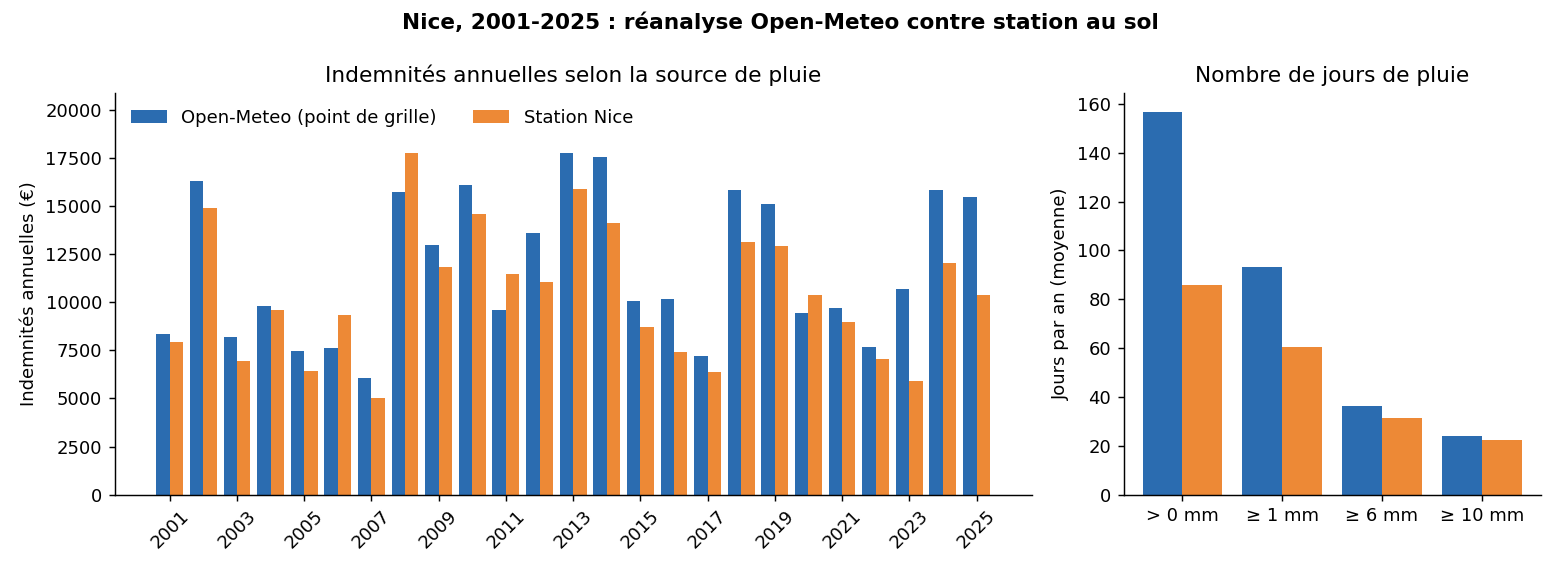
\includegraphics[width=\linewidth]{comparaison_station_nice.png}
\caption{Indemnités annuelles et nombre de jours de pluie selon la source.}
\end{figure}

\subsection{La correction du biais}\label{sec:correction}
Le logiciel corrige la pluie \textbf{avant} tout calcul, par la méthode des quantiles (\emph{quantile mapping}),
classique pour les sorties de modèles climatiques :
\[
pl_t^{\text{corrigée}} = F_{\text{station}}^{-1}\Big(F_{\text{réanalyse}}\big(pl_t\big)\Big).
\]
Chaque valeur de la réanalyse est remplacée par la valeur de la station de même rang : les bruines que la station ne
voit pas deviennent des jours secs, et les intensités autour du seuil de perte sont recalées.

\begin{itemize}
  \item \textbf{Stations} : pour chacune des 44 villes du menu, une station française à moins de 25 km avec des relevés
        complets à 85\,\% au moins ; à distance comparable, la plus complète l'emporte. \textbf{25 villes} sont calées ;
        les 19 autres (Bordeaux, Grenoble, Pau\ldots) ne sont pas corrigées et l'application le signale.
  \item \textbf{Validation honnête} : correction calée sur 2001-2013 seulement, testée sur 2014-2025.
        L'écart absolu moyen des indemnités aux stations passe de \textbf{24,1\,\% à 13,3\,\%} ; la correction améliore
        14 villes sur 25.
  \item \textbf{Activation ville par ville} : dans les 11 villes où elle a éloigné l'estimation de la station
        (Brest, Lille, Nantes, Rennes\ldots), l'interrupteur est \textbf{désactivé par défaut} ; il est activé dans les 14 autres.
  \item \textbf{Effet à Nice} : la prime commerciale passe de \eur{15\,875} à \eur{14\,183} ($-10{,}7\,\%$).
\end{itemize}

\begin{attention}
\textbf{À savoir dire à l'oral.} La table de correction est calée sur 2001-2025 puis appliquée à toutes les années :
la prime « a priori » d'une année passée comme 1998 utilise donc indirectement des relevés postérieurs. C'est assumé :
la correction ne porte que sur la \emph{forme} de la distribution des pluies, pas sur la pluie de l'année étudiée.
Pour une rétrospective strictement a priori, il suffit de désactiver la correction.
\end{attention}

% =====================================================================
\section{La tarification}

\subsection{Les 365 jours qui suivent la souscription}
Pour une souscription au 14 novembre, chaque année d'historique est découpée du 14 novembre au 13 novembre suivant.
Chaque période compte \textbf{exactement 365 jours}, comme le contrat, même si elle contient un 29 février.
On garde les $N$ dernières périodes complètes ($N = 15$ par défaut, réglable de 5 à 30). Les jours sans donnée sont
comptés comme secs et signalés ; une période où plus de 5\,\% des jours manquent est écartée.

\subsection{De la prime pure à la prime commerciale}
Sur chaque période historique on calcule l'indemnité annuelle $I = \sum_t I_t$. Puis :
\[
P_{\text{pure}} = \mathbb{E}[I] \;(\text{moyenne historique}),\qquad
P = \frac{\mathbb{E}[I] + \beta\,\sigma(I)}{1 - \alpha},
\]
avec $\sigma(I)$ l'écart-type des indemnités annuelles, $\beta = 0{,}30$ le chargement de sécurité et $\alpha = 15\,\%$
les frais de gestion et la marge. C'est le \textbf{principe de l'écart-type} : à prime pure égale, un risque irrégulier
paie plus qu'un risque stable (un test le vérifie).

\begin{encadre}
\textbf{Exemple, Nice, souscription au 14/11/2026, pluie corrigée :} $\mathbb{E}[I] = \eur{11\,146{,}27}$,
$\sigma(I) = \eur{3\,030{,}57}$, chargement $\beta\sigma = \eur{909{,}17}$, d'où
$P = (11\,146{,}27 + 909{,}17)/0{,}85 = \eur{14\,182{,}87}$.
\end{encadre}

\subsection{Pourquoi un chargement de sécurité ?}
La prime pure $\mathbb{E}[I]$ est le \textbf{coût moyen}. Un assureur qui ne ferait payer que cette moyenne serait à
l'équilibre \emph{en moyenne seulement} et perdrait de l'argent chaque année plus pluvieuse que la moyenne, sans réserve
pour l'absorber. Le chargement $\beta\,\sigma(I)$ constitue cette marge. Quatre raisons le rendent indispensable :
\begin{enumerate}
  \item \textbf{Un risque très variable} : à Nice, $\sigma(I) \approx 27\,\%$ de $\mathbb{E}[I]$. Avec la seule prime pure,
        le contrat rejoué sur 2001-2025 aurait coûté plus qu'il ne rapporte \textbf{11 années sur 25}, jusqu'à $+65\,\%$,
        et l'assureur aurait fini en perte.
  \item \textbf{Une estimation incertaine} : sur 15 ans, l'erreur type de $\mathbb{E}[I]$ vaut $\sigma/\sqrt{15} \approx 0{,}26\,\sigma$.
  \item \textbf{Un risque non mutualisable} : tous les commerçants d'une ville subissent la même pluie le même jour.
        Contrairement à l'assurance automobile, avoir plus de clients ne rend pas le total plus prévisible.
  \item \textbf{Un climat qui évolue} : une estimation sur le passé est en retard sur un risque en hausse (Brest : $+22\,\%$).
\end{enumerate}

\textbf{Pourquoi $\beta\,\sigma(I)$ (principe de l'écart-type) ?} Avec un chargement en pourcentage de la prime pure
(principe de l'espérance, notre première version), deux clients de même prime pure paieraient la même prime même si l'un
a un risque bien plus irrégulier. Avec $\beta\,\sigma(I)$, le risque irrégulier paie davantage, ce qui reflète le capital
que l'assureur doit immobiliser. L'écart-type étant en euros, $\beta$ s'interprète directement : avec $\beta = 0{,}30$, la
prime chargée correspond au 62\textsuperscript{e} centile d'une loi normale et couvre environ une erreur type d'estimation.

\textbf{Sources.} Le principe de l'écart-type $H = \mathbb{E}[S] + \rho\,\sigma(S)$ est un principe classique de calcul de
prime ; les auteurs notent le coefficient $\rho$, $\alpha$ ou $\theta$ au lieu de $\beta$ :
\begin{itemize}
  \item cours ACT2060, \emph{Calcul de la prime}, section 2.1.3 « Chargement de sécurité » :
        \url{https://bookdown.org/boucherjphilippe/ACT2060/calcul-de-la-prime.html} ;
  \item D.~Denneberg, « Premium Calculation: Why Standard Deviation Should Be Replaced by Absolute Deviation »,
        \emph{ASTIN Bulletin} 20(2), 1990, p.~181-190 :
        \url{https://www.casact.org/abstract/premium-calculation-why-standard-deviation-should-be-replaced-absolute-deviation} ;
  \item R.~Kaas, M.~Goovaerts, J.~Dhaene, M.~Denuit, \emph{Modern Actuarial Risk Theory}, Springer, chapitre
        « Premium principles and Risk measures » : \url{https://link.springer.com/10.1007/978-3-540-70998-5}.
\end{itemize}
\textbf{Limite connue} : ce principe n'est pas additif (la prime de deux risques regroupés n'est pas la somme de leurs
primes, critique de Denneberg). Sans conséquence pour tarifer un contrat seul ; pour un portefeuille, le principe de la
variance, additif pour des risques indépendants, serait préférable.

\begin{encadre}
\textbf{À dire à l'oral.} « La prime pure est une moyenne : avec elle seule, l'assureur perd de l'argent une année sur
deux et ne peut pas compenser par le nombre de clients, puisqu'ils subissent tous la même pluie. Le chargement est
proportionnel à l'écart-type : plus le risque est irrégulier, plus il coûte. »
\end{encadre}

\subsection{Pourquoi \texorpdfstring{$\beta = 0{,}30$}{beta = 0,30} ?}
L'assureur gagne de l'argent si les indemnités restent inférieures à la \textbf{prime nette de frais} $P(1-\alpha)$.
Nous avons rejoué le contrat sur 2001-2025 dans trois climats (chaque année tarifée a priori) :

\begin{table}[H]
\centering\small
\begin{tabular}{cccccc}
\toprule
$\beta$ & Nice : sinistres / prime nette & Nice : années favorables & Brest & Strasbourg & Chargement\\
\midrule
0 & 101\,\% & 44\,\% & 114\,\% & 101\,\% & 0\,\%\\
\textbf{0,30} & \textbf{93\,\%} & \textbf{36\,\%} & 107\,\% & \textbf{94\,\%} & 6 à 9\,\%\\
0,50 & 88\,\% & 24\,\% & 103\,\% & 90\,\% & 10 à 16\,\%\\
1 & 77\,\% & 8\,\% & 94\,\% & 82\,\% & 21 à 31\,\%\\
\bottomrule
\end{tabular}
\caption{Au-dessus de 100\,\%, le produit perd de l'argent. Chargement exprimé en \% de la prime pure.}
\end{table}

\begin{itemize}
  \item Sans chargement, le produit \textbf{perd de l'argent} partout : l'estimation sur le passé est en retard sur des
        années récentes plus pluvieuses.
  \item $\beta = 0{,}30$ est la plus petite valeur testée qui le rend \textbf{rentable à Nice et Strasbourg}, pour 6 à 9\,\%
        de supplément ; le client reste gagnant plus d'une année sur trois à Nice.
  \item Limite : à Brest il faudrait $\beta \approx 1$ ; le curseur permet d'ajuster $\beta$ par région.
\end{itemize}

\subsection{Pourquoi 15 années d'historique ?}
Le choix de $N$ est un compromis : \textbf{trop peu d'années, trop de hasard} (l'incertitude sur la prime pure vaut
$\sigma(I)/\sqrt{N}$) ; \textbf{trop d'années, un retard sur le climat} (à Brest, les indemnités moyennes ont augmenté de
22\,\% entre 1971-1995 et 2001-2025). Le contrat a été rejoué sur 2001-2025 avec $N$ de 5 à 30 ans ; la précision est
l'écart entre la prime pure d'une année et les indemnités réellement versées en moyenne sur les 5 années suivantes.

\begin{table}[H]
\centering\small
\begin{tabular}{cccc}
\toprule
$N$ & Erreur de prédiction (3 villes) & Variation annuelle de la prime & Sous-estimation à Brest\\
\midrule
5 & 17,5\,\% & 4,5 à 7,7\,\% & 5\,\%\\
10 & 15,5\,\% & 2,9 à 3,4\,\% & 10\,\%\\
\textbf{15} & \textbf{12,6\,\%} & \textbf{1,6 à 2,3\,\%} & 12\,\%\\
20 & 13,0\,\% & 1,2 à 2,0\,\% & 14\,\%\\
30 & 13,6\,\% & 1,0 à 1,3\,\% & 15\,\%\\
\bottomrule
\end{tabular}
\caption{Contrat rejoué sur 2001-2025 à Nice, Brest et Strasbourg selon la longueur d'historique.}
\end{table}

15 ans donne la plus faible erreur de prédiction, avec une prime déjà stable ; au-delà, on ne gagne presque plus en
stabilité mais on suit moins bien le climat. L'écart avec 20 ans est faible : les deux se valent, 15 est retenu pour
mieux suivre l'évolution du climat.

\begin{encadre}
\textbf{À dire à l'oral.} « Avec 5 ans, la prime dépend trop du hasard ; avec 30 ans, elle est en retard sur le climat.
Testé sur 25 ans dans trois villes, 15 ans donne la meilleure prédiction avec une prime stable. »
\end{encadre}

\subsection{La VaR 95 \% : affichée, mais fragile}
La VaR 95\,\% (indemnités dépassées une année sur vingt) est affichée à titre indicatif. Avec 15 années, ce centile
repose presque entièrement sur les deux plus fortes années : selon la fenêtre choisie, il varie de $+19\,\%$ à Nice et de
$+46\,\%$ à Brest. C'est pourquoi \textbf{elle n'entre pas dans la prime}, qui repose sur la moyenne et l'écart-type.

% =====================================================================
\section{Le devis}
Une fois la prime calculée, le client saisit son nom et sa raison sociale et télécharge un \textbf{devis PDF} :
bloc assureur (« Météo Assur », assureur fictif), référence unique \texttt{DEV-AAAAMMJJ-XXXXXX}, date de validité (30 jours),
données du souscripteur, dates de couverture, garantie, source météo, détail de la prime (pure, sécurité, frais) et une
zone de signature pour chaque partie. Si un paramètre change après le calcul, le devis est masqué jusqu'au recalcul :
un devis ne peut jamais associer un profil à la prime d'un autre.

\begin{figure}[H]
\centering
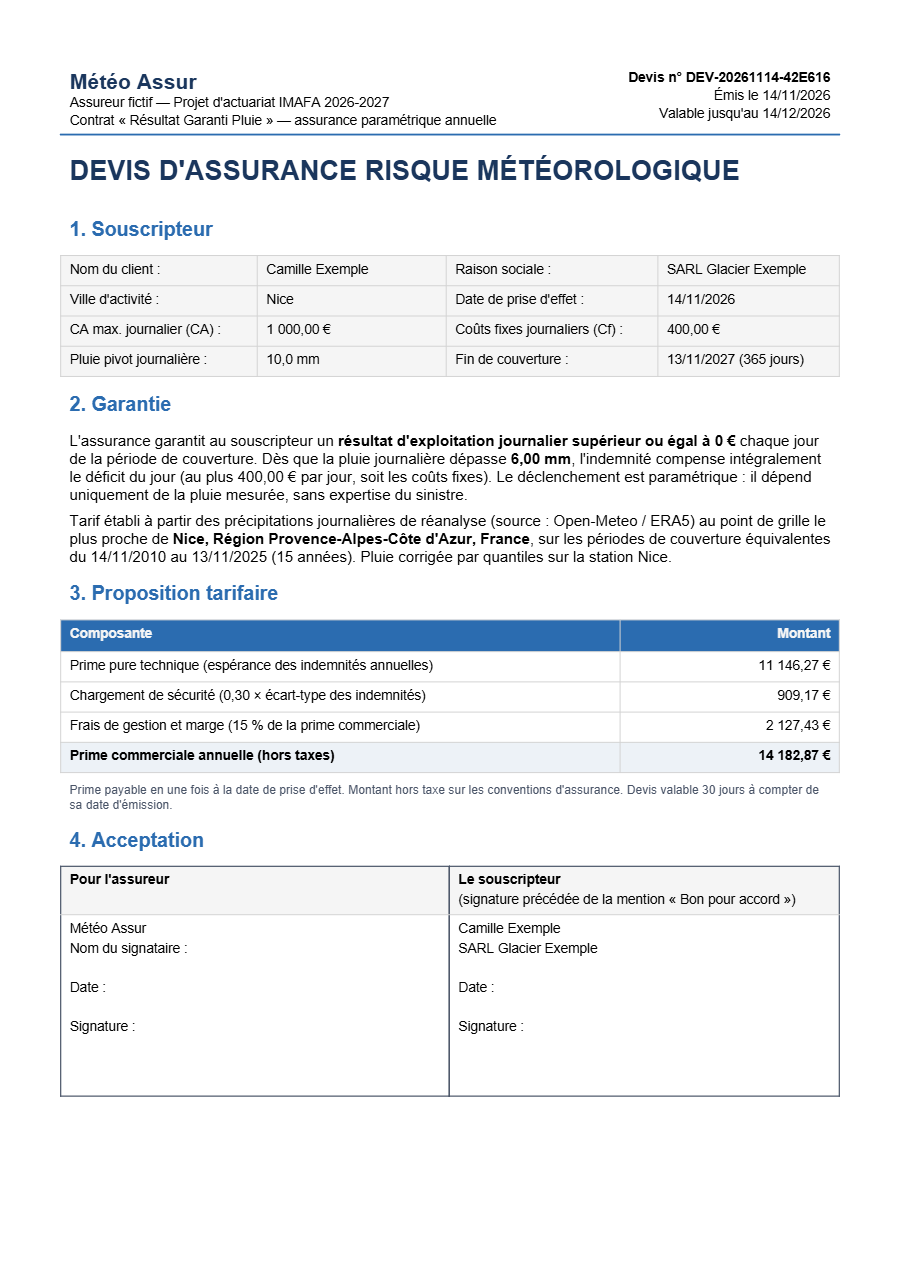
\includegraphics[width=0.62\linewidth]{capture_devis.png}
\caption{Devis généré par l'application (client fictif).}
\end{figure}

% =====================================================================
\section{L'analyse rétrospective}\label{sec:retro}

\subsection{Une année passée}
Pour une année $a$, la prime $P_a$ est \textbf{calculée par le logiciel}, comme au 1\textsuperscript{er} janvier de $a$,
avec les seules années antérieures. Elle est ensuite comparée à ce qui s'est réellement passé pendant $a$.

\begin{encadre}
\textbf{Nice 1998} (profil par défaut, historique 1983-1997, pluie corrigée) :
prime a priori $P_{1998} = \eur{12\,746}$ ; $R_{nass} = \eur{188\,902}$ ; $R_{ass} = \eur{196\,610}$ ;
pertes évitées \eur{7\,708} ; $R_{net} = \eur{183\,864}$. \textbf{S'assurer n'aurait pas été favorable} ($-\eur{5\,038}$) :
1998 a été moins pluvieuse que la moyenne des quinze années précédentes.
\end{encadre}

\subsection{Plusieurs années}
Chaque année d'une plage (2001-2025 par défaut) est tarifée a priori puis comparée aux indemnités versées.
À Nice : \textbf{ratio sinistres / primes de 79\,\%} (rentable pour l'assureur) et assurance favorable au client
\textbf{36\,\% des années}. La prime est une moyenne : trop chère les années sèches, avantageuse les années pluvieuses.
C'est exactement ce que l'analyse rétrospective sert à montrer.

\begin{figure}[H]
\centering
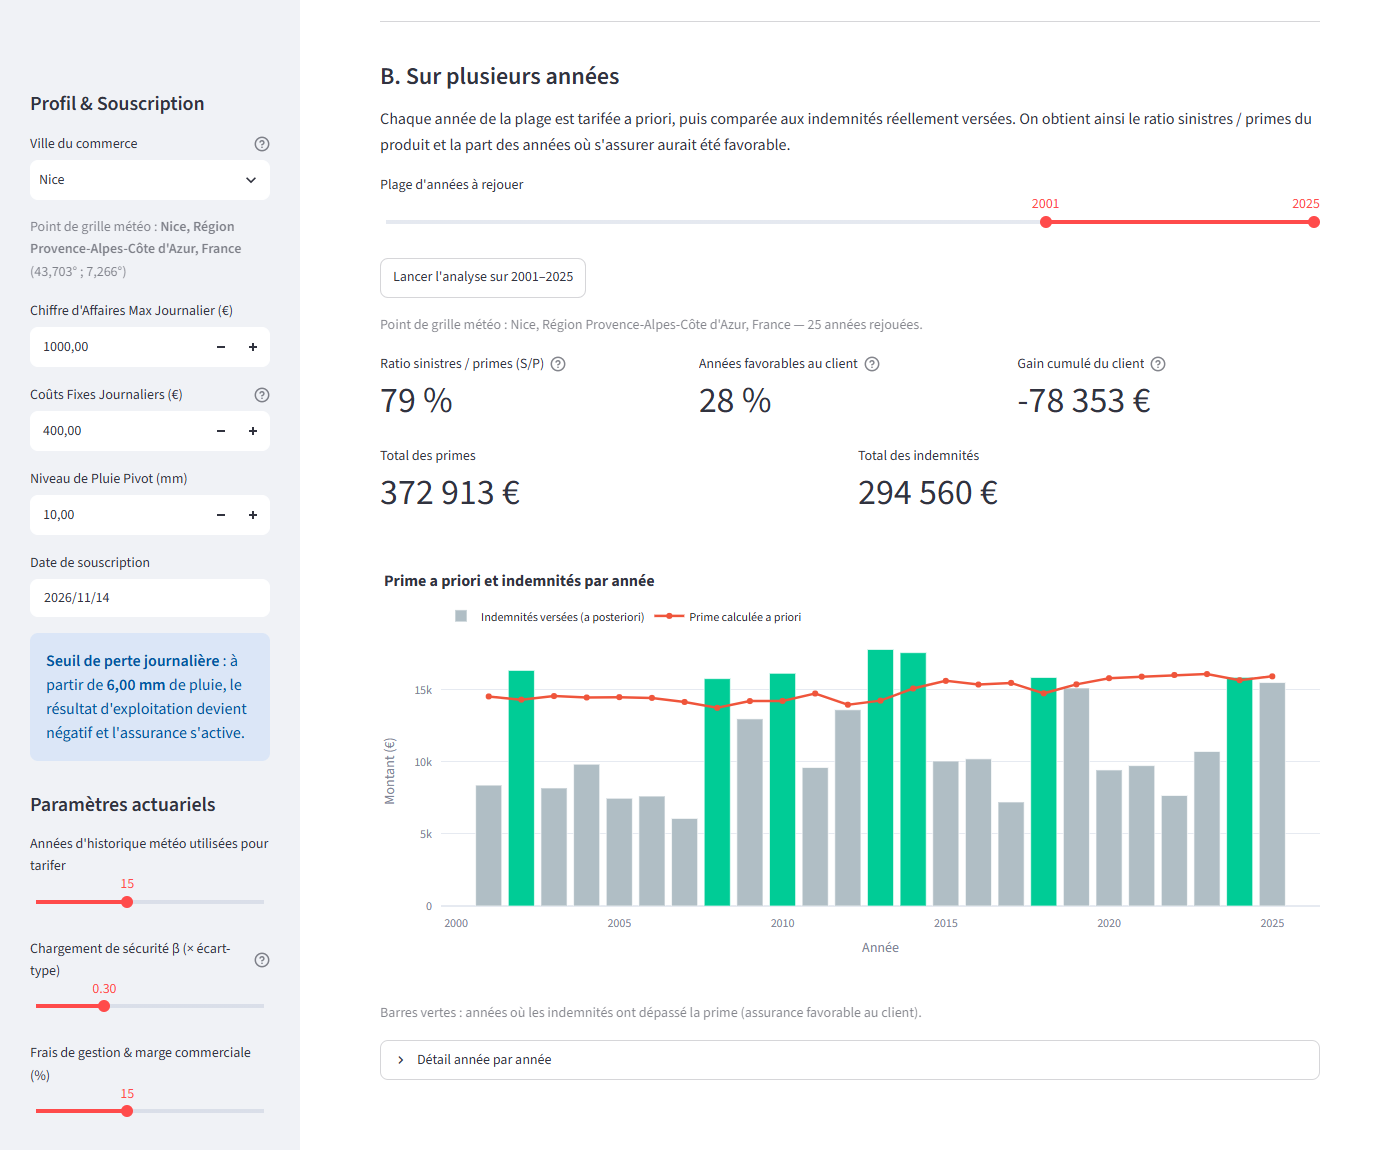
\includegraphics[width=0.9\linewidth]{capture_retrospective_plusieurs_annees.png}
\caption{Analyse sur 2001-2025 : barres vertes = années favorables au client.}
\end{figure}

% =====================================================================
\section{Le logiciel}

\subsection{L'interface}
Application web \textbf{Streamlit} en trois onglets (Tarification \& devis, Analyse rétrospective, Guide), avec le profil
du client et les paramètres actuariels dans la barre latérale. Elle est en ligne, s'affiche correctement sur téléphone
(barre latérale repliée, colonnes empilées) et sur tablette, et les montants sont au format français.

\begin{figure}[H]
\centering
\begin{minipage}{0.70\linewidth}\centering
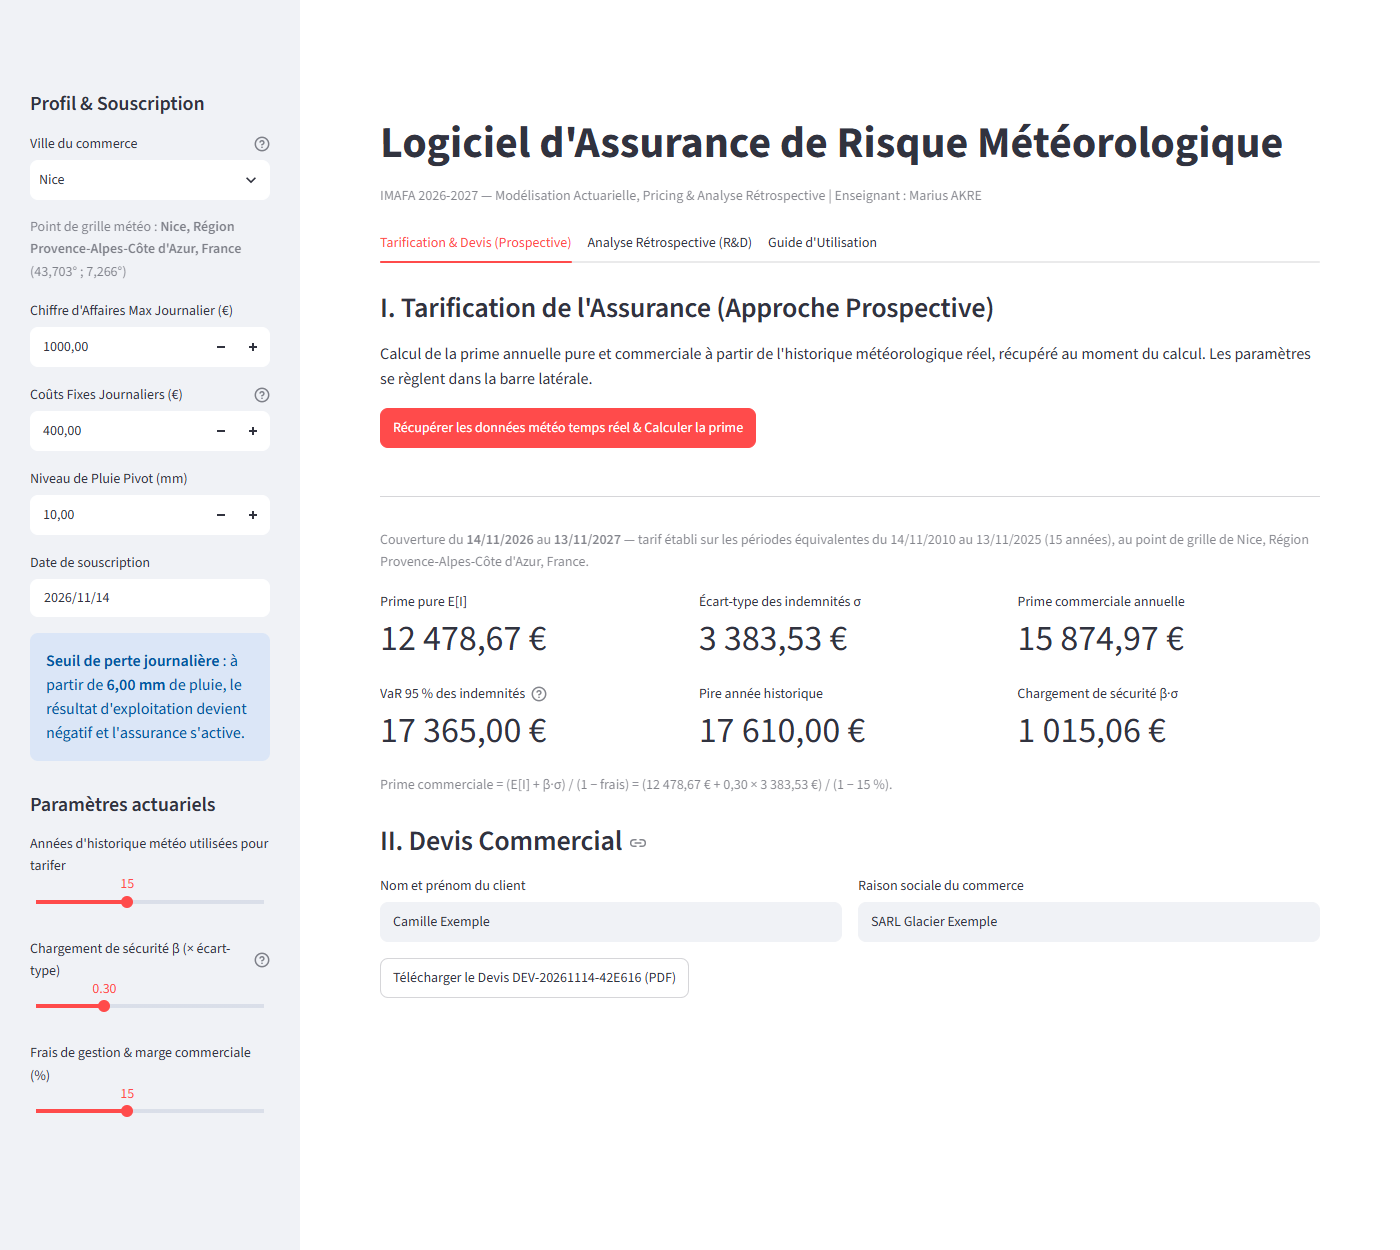
\includegraphics[width=\linewidth]{capture_tarification.png}
\end{minipage}\hfill
\begin{minipage}{0.26\linewidth}\centering
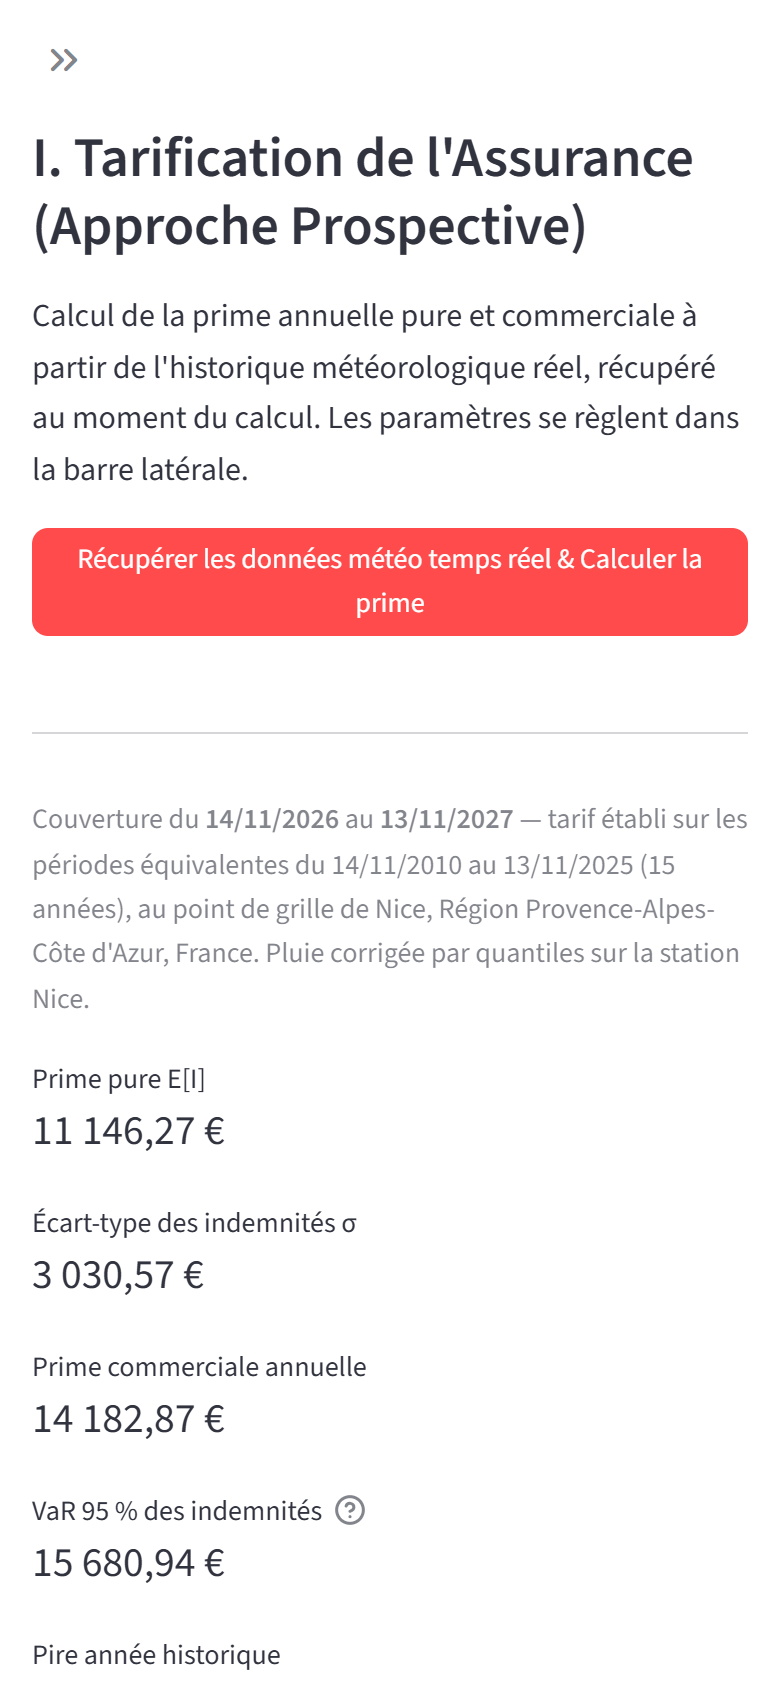
\includegraphics[width=\linewidth]{capture_mobile.png}
\end{minipage}
\caption{Onglet Tarification sur ordinateur (à gauche) et sur téléphone (à droite).}
\end{figure}

\subsection{L'organisation du code}
\begin{table}[H]
\centering\small
\begin{tabularx}{\linewidth}{>{\ttfamily}lX}
\toprule
\normalfont Fichier & Rôle\\
\midrule
app.py & Interface Streamlit\\
src/simulation.py & Formules du sujet : CA, résultat, indemnité journaliers\\
src/pricing.py & Périodes de 365 jours, prime pure, écart-type, VaR, chargements\\
src/backtesting.py & Analyse rétrospective sur une ou plusieurs années\\
src/weather\_api.py & Géocodage et pluie Open-Meteo (nouvelles tentatives, erreurs lisibles)\\
src/bias\_correction.py & Correction par quantiles, calée sur les stations\\
src/pdf\_generator.py & Devis PDF\\
src/visualisations.py & Graphiques Plotly\\
src/formatting.py & Montants au format français\\
src/cities.py & Villes du menu déroulant\\
data/calibration\_stations.json & Tables de correction des 25 villes calées\\
notebooks/ & Démonstration pas à pas, exécutée, avec ses graphiques\\
scripts/ & Calage de la correction, comparaison avec la station, génération du guide PDF\\
tests/ & 32 tests automatiques, hors connexion\\
\bottomrule
\end{tabularx}
\end{table}

\subsection{Qualité et robustesse}
\begin{itemize}
  \item \textbf{32 tests automatiques} (\texttt{python -m pytest tests/}), dont l'exemple chiffré du sujet reproduit
        exactement et un test sur la vraie pluie de Nice 1998, sans connexion.
  \item En cas de panne de l'API météo, 3 tentatives puis un message clair au lieu d'un plantage.
  \item Les résultats restent affichés tant que les paramètres ne changent pas ; sinon, un message invite à relancer.
\end{itemize}

\subsection{L'accès en ligne}
\begin{minipage}{0.72\linewidth}
L'application est hébergée gratuitement sur Streamlit Community Cloud, depuis la branche \texttt{main} de la fork de
Tahitoa. Chaque mise à jour de \texttt{main} chez Amiel doit être suivie d'un clic sur « Sync fork » pour que l'application
en ligne suive. Après quelques jours sans visite, elle se met en veille : \textbf{l'ouvrir une heure avant la présentation}.
\end{minipage}\hfill
\begin{minipage}{0.22\linewidth}\centering

\includegraphics[width=\linewidth]{qr_application.png}
\end{minipage}

% =====================================================================
\section{Ce que nous avons fait, étape par étape}

\begin{enumerate}[leftmargin=*]
  \item \textbf{Première version} : modèle, tarification, devis et rétrospective en Streamlit, données Open-Meteo.
  \item \textbf{Conformité au sujet} : la prime rétrospective était saisie à la main (\eur{3\,000}) ; elle est désormais
        \textbf{calculée a priori}. La date de souscription est réellement utilisée (365 jours qui suivent).
  \item \textbf{Fiabilité} : devis bloqué si le profil change, pannes réseau gérées, jours manquants signalés, plantage
        corrigé quand $CA < \eur{400}$.
  \item \textbf{Interface} : menu de 44 villes avec saisie libre, emojis retirés, montants lisibles à toutes les largeurs.
  \item \textbf{Approfondissement actuariel} : chargement $\beta\sigma$ au lieu d'un pourcentage fixe, VaR affichée,
        rétrospective sur plusieurs années (ratio sinistres / primes), justification de $\beta$ par backtest.
  \item \textbf{Devis complet} : client, assureur, validité, signatures.
  \item \textbf{Mise en ligne} : déploiement Streamlit, lien et QR code, captures d'écran, guide en PDF.
  \item \textbf{Fusion avec le travail de l'équipe} : intégration du README, du notebook et des données de \texttt{main} ;
        retrait des secours silencieux (ville inconnue remplacée par Nice, pluie de 1998 renvoyée sans réseau).
  \item \textbf{Source météo} : comparaison avec la station de Nice, puis correction par quantiles validée hors échantillon,
        activée seulement là où elle aide.
\end{enumerate}

% =====================================================================
\section{Préparer l'oral}

\subsection{Déroulé conseillé (10 minutes)}
\begin{enumerate}
  \item Le besoin et le modèle (1 min 30) : formules, seuil de 6 mm, indemnité = perte du jour.
  \item Démonstration en ligne (4 min) : profil, prime, devis PDF, rétrospective 1998 puis 2001-2025.
  \item Choix actuariels (2 min) : $\beta\sigma$ et sa justification, VaR indicative.
  \item Source météo (2 min) : biais de la réanalyse, correction et sa validation.
  \item Limites et pistes (30 s).
\end{enumerate}

\subsection{Questions probables du jury}
\begin{description}[style=nextline,leftmargin=0pt]
  \item[Pourquoi vos chiffres de 1998 ne sont-ils pas ceux du sujet ?]
    Les montants du sujet sont illustratifs ; nous utilisons la vraie météo de Nice. Nos tests reproduisent exactement
    l'exemple du sujet sur une année construite pour donner ces montants.
  \item[La prime de 1998 est-elle vraiment calculée a priori ?]
    Oui, avec les seules années 1983-1997. Seule la table de correction utilise des relevés plus récents, ce que nous
    assumons ; sans correction, le calcul est strictement a priori.
  \item[Pourquoi l'assurance est-elle souvent défavorable au client ?]
    La prime est une moyenne chargée : elle est donc supérieure aux indemnités la plupart des années, et inférieure les
    années très pluvieuses. C'est le principe même de l'assurance ; sinon l'assureur perdrait de l'argent.
  \item[Pourquoi ne pas utiliser directement les stations ?]
    Elles ne couvrent pas toutes les villes et ne sont pas toujours disponibles en temps réel ; la réanalyse couvre tout le
    territoire. La correction combine les deux : la couverture de la réanalyse, la justesse de la station.
  \item[Pourquoi la VaR n'est-elle pas dans la prime ?]
    Estimée sur 15 années, elle dépend des deux pires années et varie de près de 50\,\% selon la période.
\end{description}

\subsection{Limites et pistes}
\begin{itemize}
  \item Le modèle de chiffre d'affaires est celui du sujet (linéaire, sans saisonnalité ni effet week-end).
  \item $\beta$ unique alors qu'il devrait dépendre du climat (Brest) ; un $\beta$ par région serait une suite naturelle.
  \item La correction n'est disponible que pour 25 villes et reste imparfaite (léger surcoût résiduel en moyenne).
  \item Un produit réel déclencherait l'indemnité sur une station officielle de référence, définie au contrat.
\end{itemize}

\end{document}
